% !TEX TS-program = pdflatex
% !TEX encoding = UTF-8 Unicode

% This is a simple template for a LaTeX document using the "article" class.
% See "book", "report", "letter" for other types of document.

\documentclass[10pt]{article} % use larger type; default would be 10pt

\usepackage[utf8]{inputenc} % set input encoding (not needed with XeLaTeX)

%%% Examples of Article customizations
% These packages are optional, depending whether you want the features they provide.
% See the LaTeX Companion or other references for full information.

%%% PAGE DIMENSIONS
\usepackage{geometry} % to change the page dimensions
\geometry{letterpaper} % or letterpaper (US) or a5paper or....
\geometry{margin=1in} % for example, change the margins to 2 inches all round
% \geometry{landscape} % set up the page for landscape
%   read geometry.pdf for detailed page layout information

\usepackage{graphicx} % support the \includegraphics command and options
\usepackage{mathrsfs}
% \usepackage[parfill]{parskip} % Activate to begin paragraphs with an empty line rather than an indent

%%% PACKAGES
\usepackage{booktabs} % for much better looking tables
\usepackage{array} % for better arrays (eg matrices) in maths
\usepackage{paralist} % very flexible & customisable lists (eg. enumerate/itemize, etc.)
\usepackage{verbatim} % adds environment for commenting out blocks of text & for better verbatim
\usepackage{subfig} % make it possible to include more than one captioned figure/table in a single float
\usepackage[font=small,labelfont=bf]{caption} % Required for specifying captions to tables and figures
% These packages are all incorporated in the memoir class to one degree or another...

%%% HEADERS & FOOTERS
\usepackage{fancyhdr} % This should be set AFTER setting up the page geometry
\pagestyle{fancy} % options: empty , plain , fancy
\renewcommand{\headrulewidth}{0pt} % customise the layout...
\lhead{}\chead{}\rhead{}
\lfoot{}\cfoot{\thepage}\rfoot{}

%%% SECTION TITLE APPEARANCE
\usepackage{sectsty}
\allsectionsfont{\sffamily\mdseries\upshape} % (See the fntguide.pdf for font help)
% (This matches ConTeXt defaults)

%%% ToC (table of contents) APPEARANCE
\usepackage[nottoc,notlof,notlot]{tocbibind} % Put the bibliography in the ToC
\usepackage[titles,subfigure]{tocloft} % Alter the style of the Table of Contents
\renewcommand{\cftsecfont}{\rmfamily\mdseries\upshape}
\renewcommand{\cftsecpagefont}{\rmfamily\mdseries\upshape} % No bold!
\newcommand{\centerfig}[2]{\begin{center}\includegraphics[width=#1\textwidth]{#2}\end{center}}
\usepackage{amssymb}
\usepackage{mathtools}
\DeclarePairedDelimiter\ceil{\lceil}{\rceil}
\DeclarePairedDelimiter\floor{\lfloor}{\rfloor}
\let\oldemptyset\emptyset
\let\emptyset\varnothing
\usepackage[usenames, dvipsnames]{color}
\makeatletter
\def\@maketitle{%
  \newpage
  \null
  \vskip 1em%
  \begin{center}%
  \let \footnote \thanks
	\vskip -5em%
    {\LARGE \@title \par}%
    \vskip 1em
    {\large
      \lineskip .5em%
      \begin{tabular}[t]{c}%
        \@author
      \end{tabular}\par}%
    \vskip 1em%
    {\large \@date}%
  \end{center}%
  \par
  \vskip 1.5em}
\makeatother
%%% END Article customizations

%%% The "real" document content comes below...

\title{Physics 410: Project 2}
\author{Arnold Choa -- 32038144}
\date{12 November, 2018} % Activate to display a given date or no date (if empty),
         % otherwise the current date is printed 
%{\color{red}{\normalsize{\textbf{TODO}}}} %TODO signage
\begin{document}
\maketitle
Please see \texttt{ising2D.py} in the code folder for the base 2d Ising model code. It returns \texttt{Elist} and \texttt{Mlist} instead of the $<E>$ and $<M>$ just so that the rest of the project has a common denominator of results to work with.

Firstly, to interpolate our 1D Ising model into a 2D Ising model, we need to make come changes:
\begin{itemize}
	\item $t \sim N^2$, since the number of steps should be  proportional to the number of atoms in our lattice
	\item $E(\{\sigma \}) = -J\left(\sum_{j=1}^{N}\sum_{i=1}^{N} \sigma_{i,j}\sigma_{i,j+1}\right) -J\left(\sum_{j=1}^{N}\sum_{i=1}^{N} \sigma_{i,j}\sigma_{i+1,j}\right)$. This accounts for both horizontal and vertical coupling. This form also allows for a further generalization if vertical and horizontal coupling are different.
	\item Instead of \texttt{trials}, we have \texttt{trialsh} and \texttt{trialsv} to allow us to choose uniformly on a lattice.
	\item Instead of just left and right, we now also have up and down neighbors. We will not be taking into account the diagonal neighbors since those would be second-nearest 
neighbors.
	\item $dE = 2J\sigma_{i,j}\left(\sigma_{i,j-1} + \sigma_{i,j+1}\right) + 2J\sigma_{i,j}\left(\sigma_{i-1,j} + \sigma_{i+1,j}\right)$ to now account the 2nd dimension.
\end{itemize}

Relevant code for the next sections should be found in the \texttt{main.py} in the code folder.

Comparing the average number of spin flips needed for lattices of $N=20$ and $N=40$ ($J=1$ and $T=3$) to thermalize, we can be seen that the smaller lattice ($N=20$) thermalizes faster than the $N=40$. The $N=20$ lattice takes around $4,000$ spin flips to thermalize while the $N=40$ lattice takes around $12,000$ spin flips to thermalize. Also calculating for a $N=80$ lattice, we can see that that configuration take around $60,000$ spin flips to thermalize. We can say thermalization time seems to increase linearly with lattice size (number of atoms).
\begin{center}
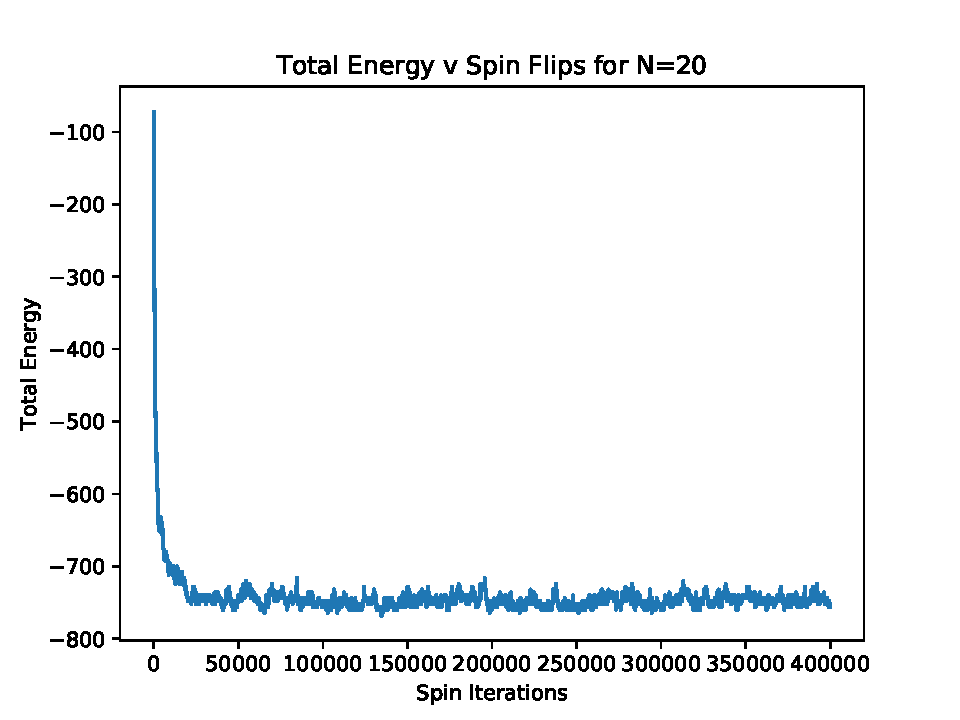
\includegraphics[width=.3\textwidth]{../figs/q2_N20.pdf}
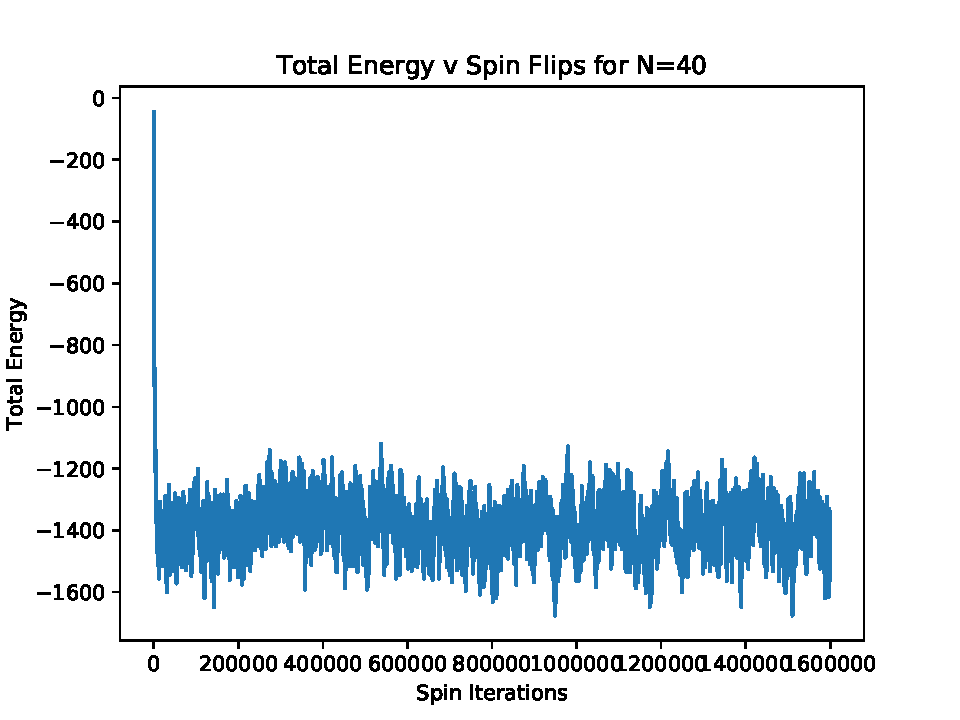
\includegraphics[width=.3\textwidth]{../figs/q2_N40.pdf}
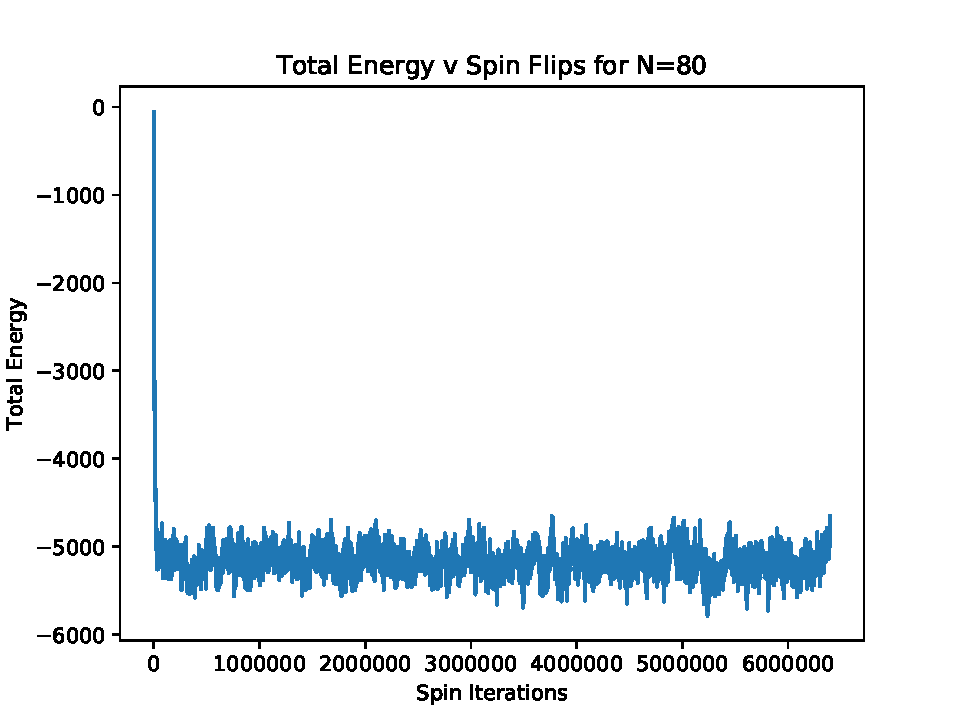
\includegraphics[width=.3\textwidth]{../figs/q2_N80.pdf}
\end{center}

For the next couple of plots, I will assume that $J=1$ for convenience and consistency with the last section.

I plot the quantities of total energy, magnetization, heat capacity, and magnetic susceptibility:

\begin{tabular}{p{2cm} | >{\centering\arraybackslash}m{5cm} >{\centering\arraybackslash}m{5cm} >{\centering\arraybackslash}m{5cm}}
	& N=10 & N=20 & N = 50 \\
\hline & & & \\
Total Energy & 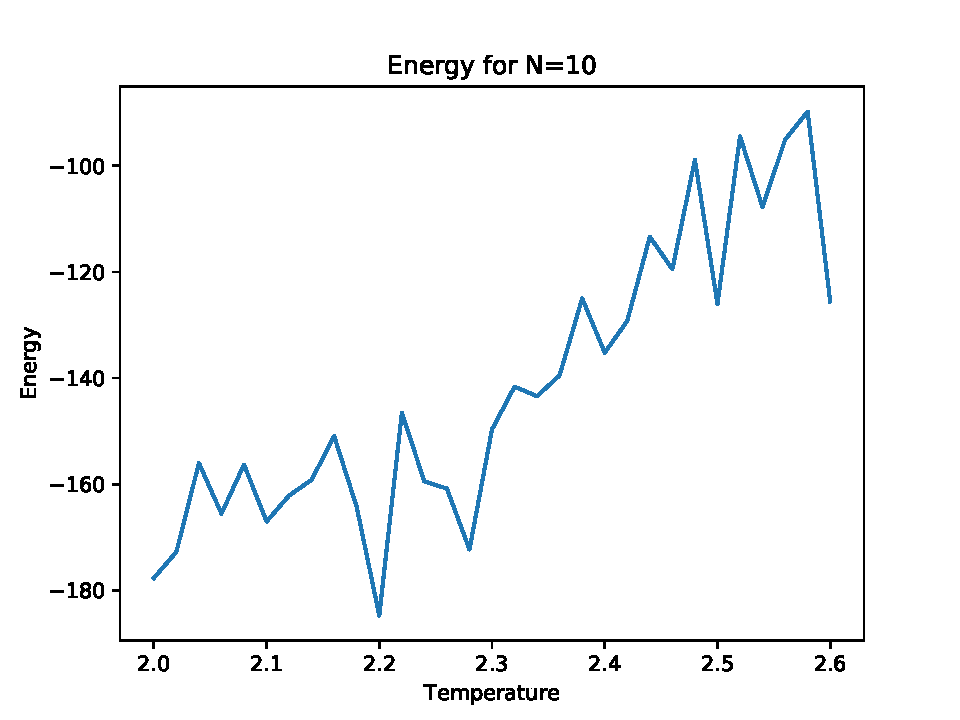
\includegraphics[width=.3\textwidth]{../figs/q3_N10_EL.pdf} & 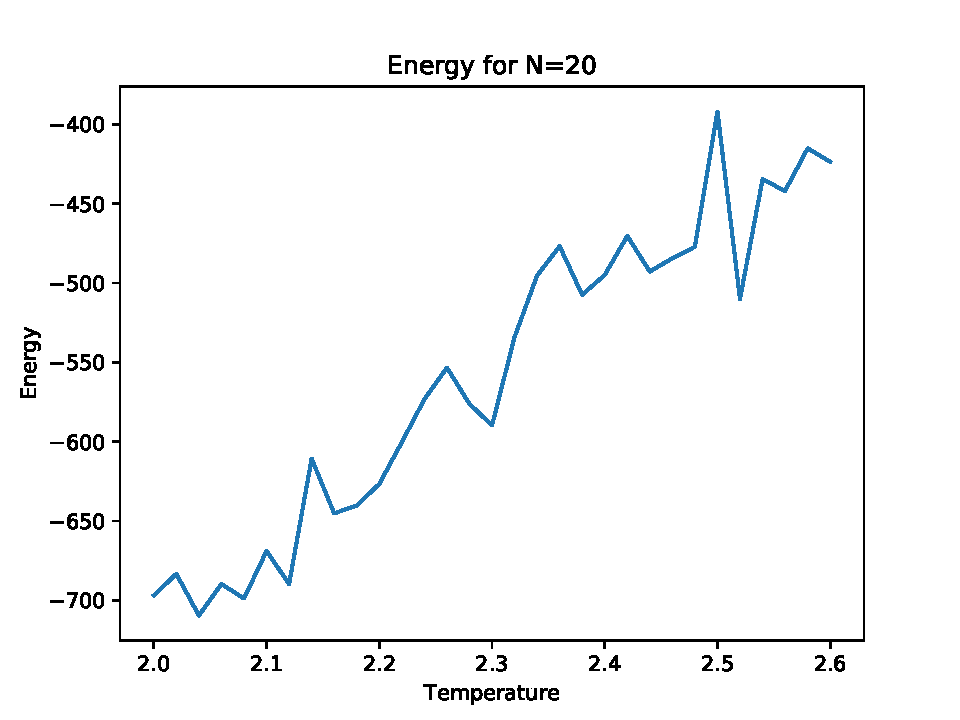
\includegraphics[width=.3\textwidth]{../figs/q3_N20_EL.pdf} & 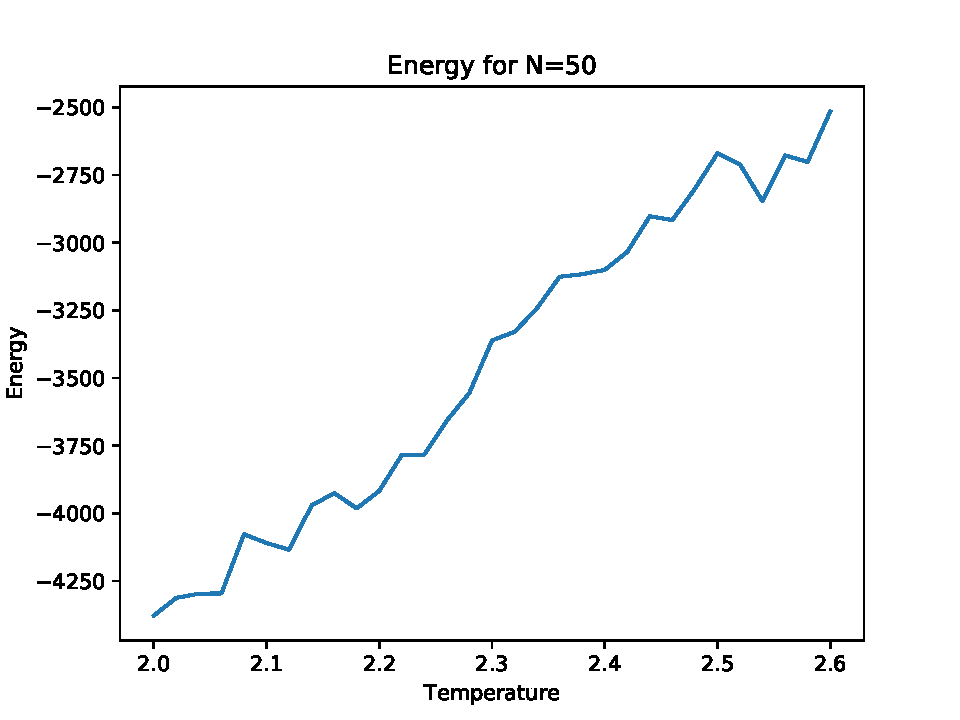
\includegraphics[width=.3\textwidth]{../figs/q3_N50_EL.pdf} \\
Total Magnetization & 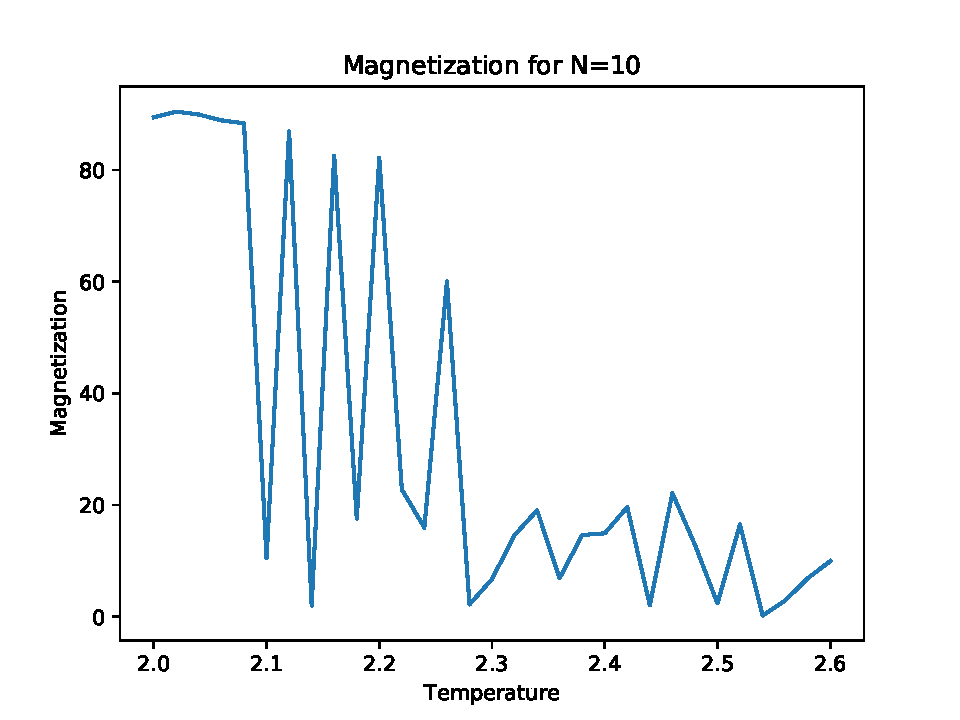
\includegraphics[width=.3\textwidth]{../figs/q3_N10_ML.pdf} & 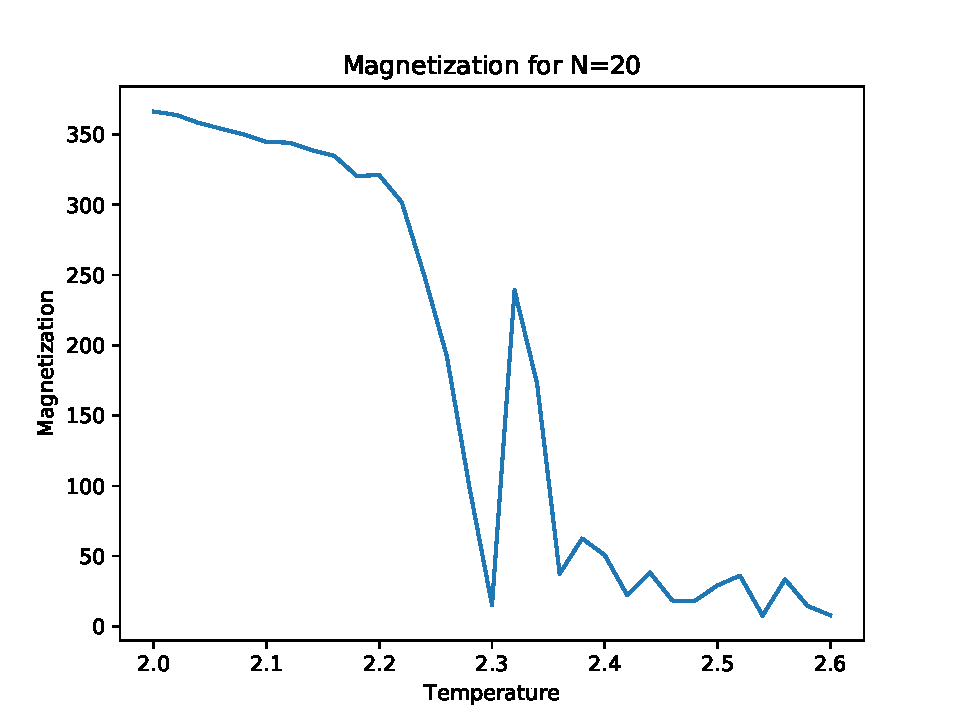
\includegraphics[width=.3\textwidth]{../figs/q3_N20_ML.pdf} & 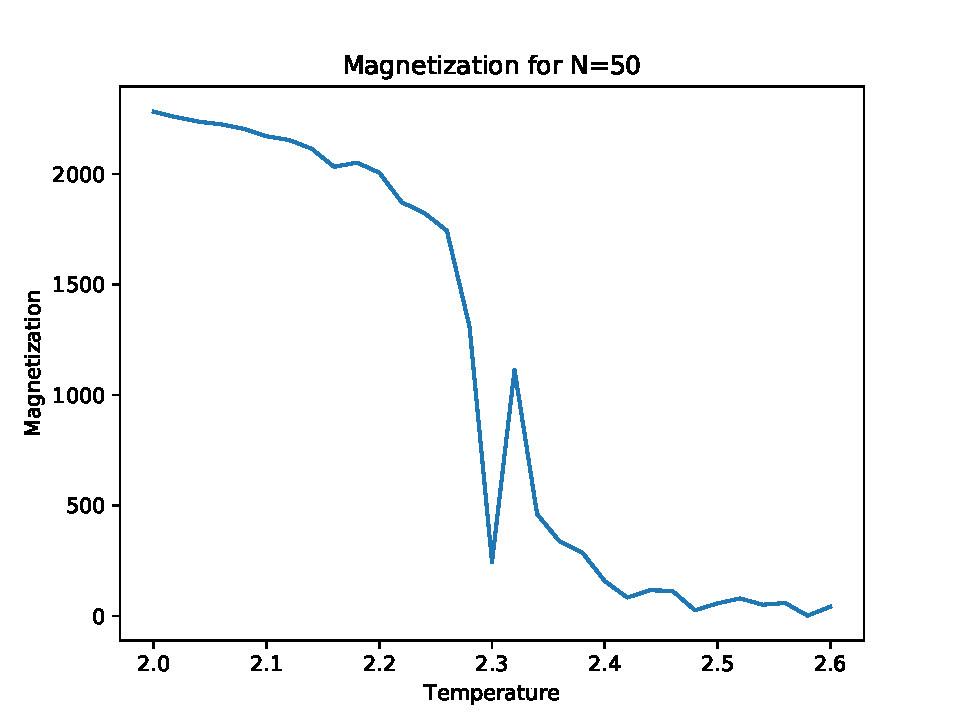
\includegraphics[width=.3\textwidth]{../figs/q3_N50_ML.pdf} \\
Heat Capacity & 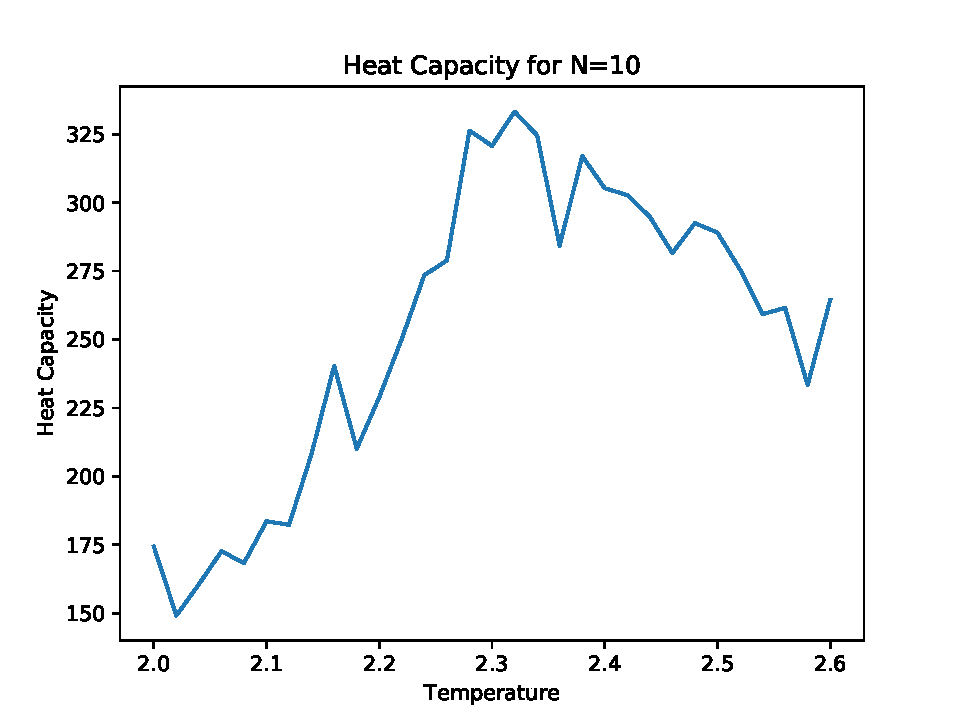
\includegraphics[width=.3\textwidth]{../figs/q3_N10_C.pdf} & 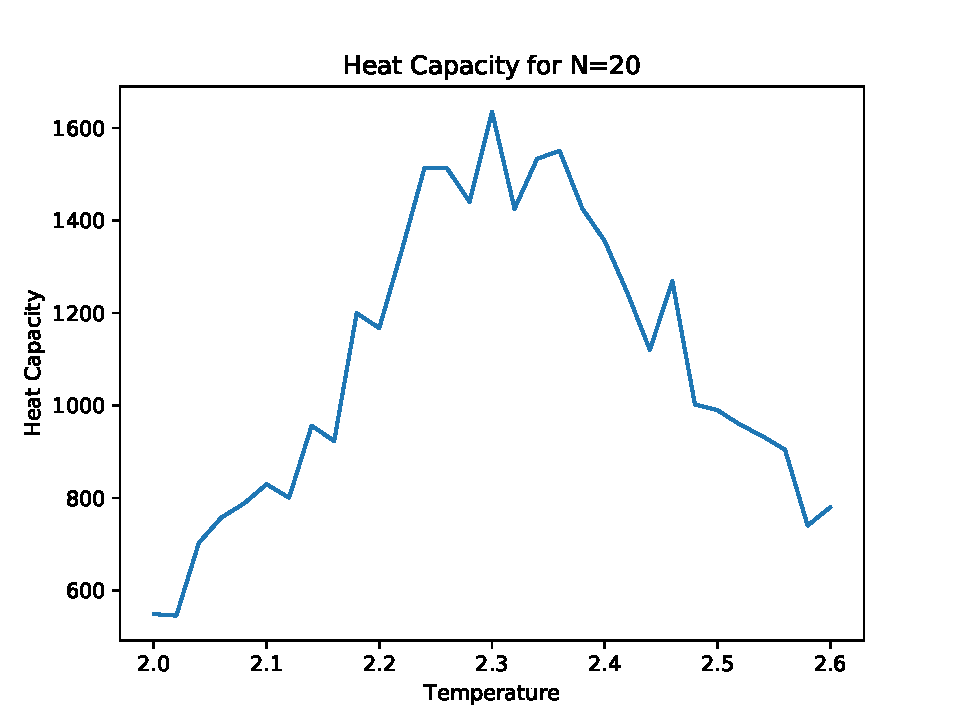
\includegraphics[width=.3\textwidth]{../figs/q3_N20_C.pdf} & 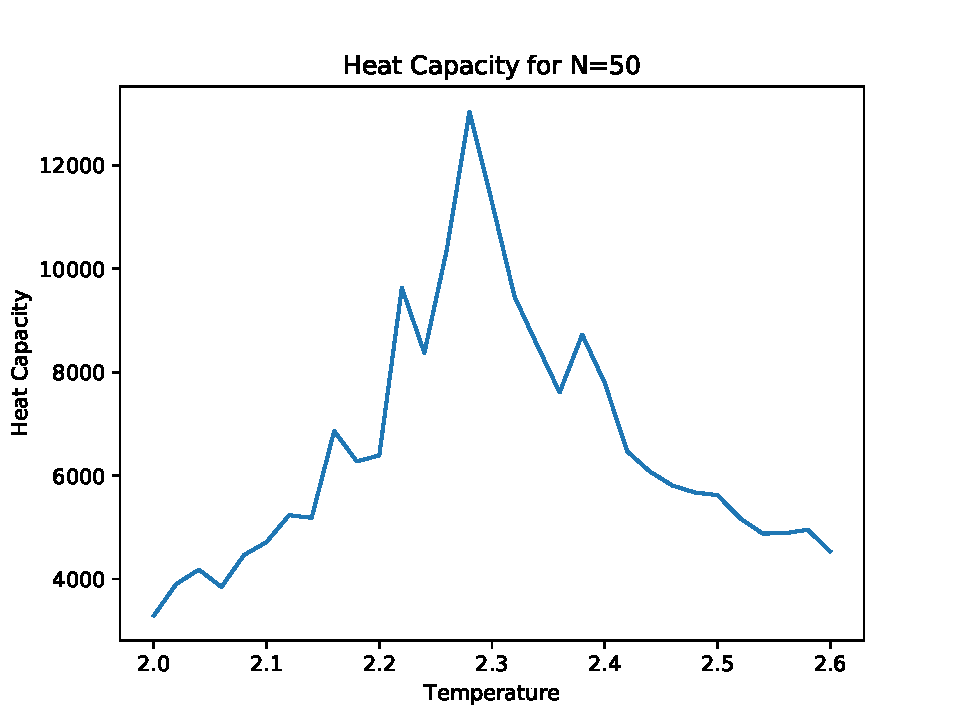
\includegraphics[width=.3\textwidth]{../figs/q3_N50_C.pdf} \\
Magnetic Susceptibility & 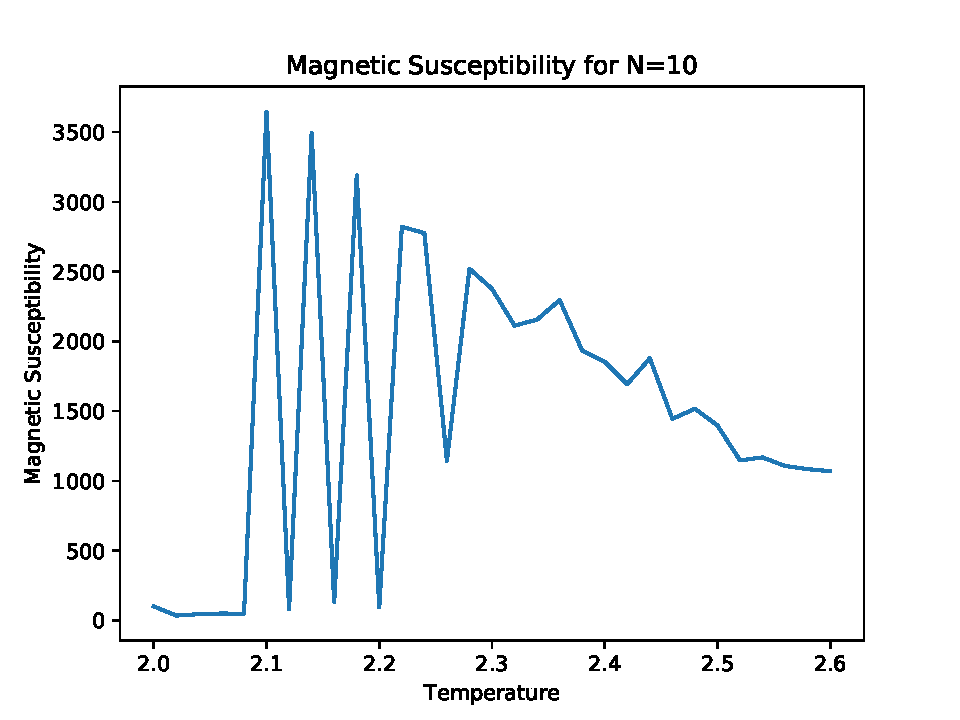
\includegraphics[width=.3\textwidth]{../figs/q3_N10_X.pdf} & 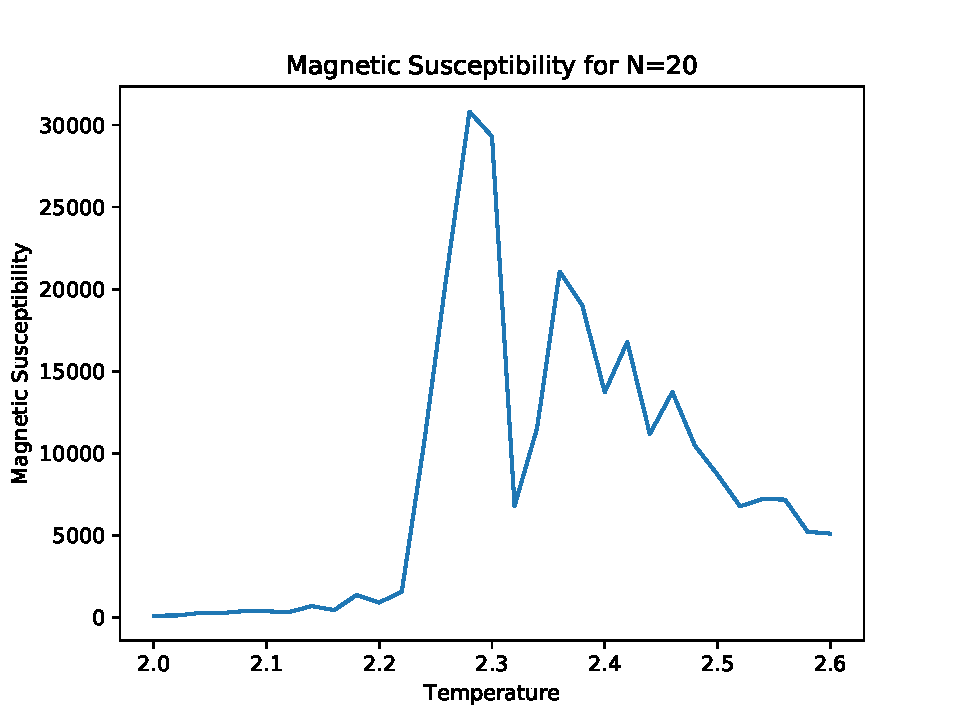
\includegraphics[width=.3\textwidth]{../figs/q3_N20_X.pdf} & 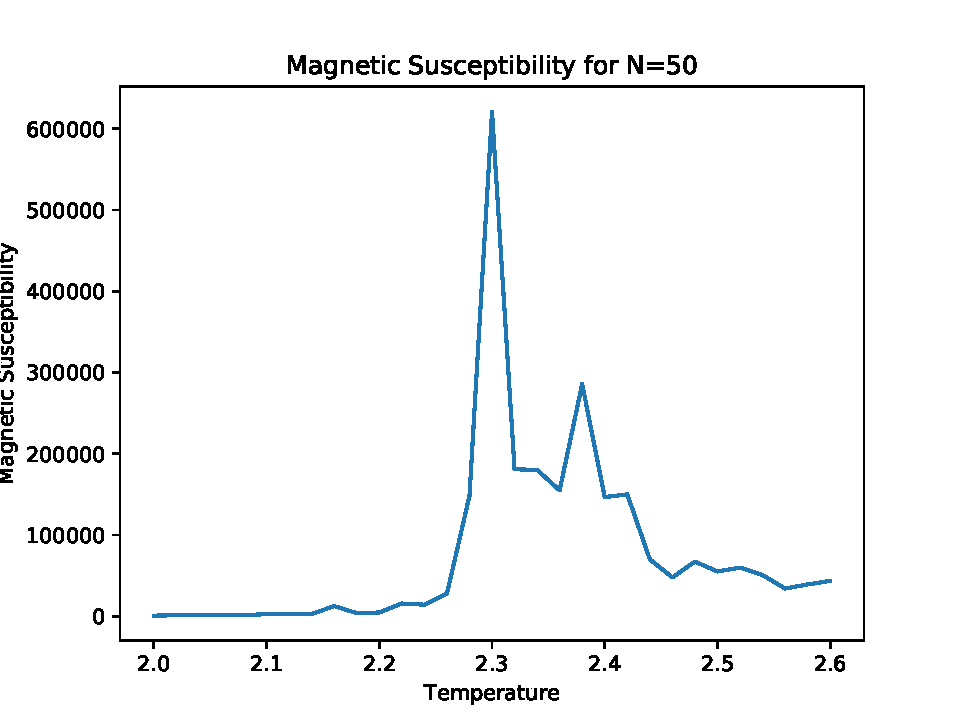
\includegraphics[width=.3\textwidth]{../figs/q3_N50_X.pdf} \\
\end{tabular}

As we can see, accuracy of the approximations of the various quantities increase as the lattice size increases. This is mostly because we are getting more and more disordered in our calculations. When we were at $N=10$, everytime we would flip $1$ spin, we would be flipping every $1$ out of a $100$ spins, while when we were at $N=50$, everytime we would flip $1$ spin, we would be flipping every $1$ out of a $2500$ spins whicch is a better approximation of disorder. At the asymptotic limit, as $N \rightarrow \infty$, we would get the best approximation at each Temperature (though at that point, we would also have an enormously big runtime).

As for the approximate location of the phase transition, we take the $50x50$ lattice with a smaller step size to better approximation of calculation and resolution of the curve. Since the Curie Temperature is characterized to be the temperature where the Magnetization drastically drops to 0, we can use the magnetic susceptibility to see where the largest change in magnetization happens. We can also use the Heat capacity since a drastic change in Magnetization also makes a drastic change in Energy of the lattice.
\begin{center}
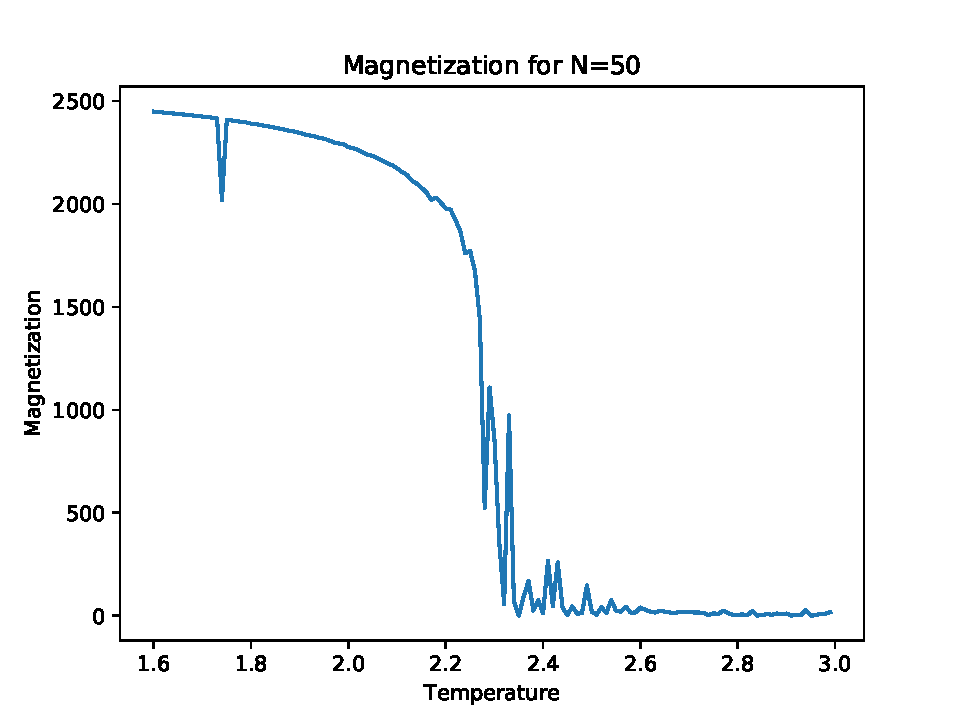
\includegraphics[width=.3\textwidth]{../figs/q4_N50_ML.pdf}
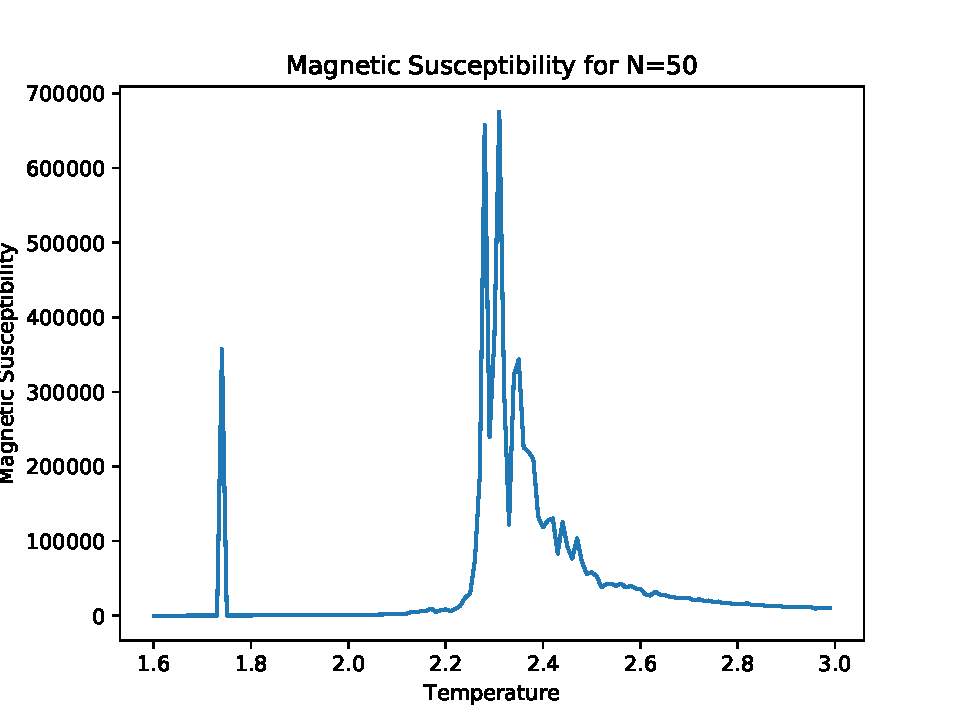
\includegraphics[width=.3\textwidth]{../figs/q4_N50_X.pdf}
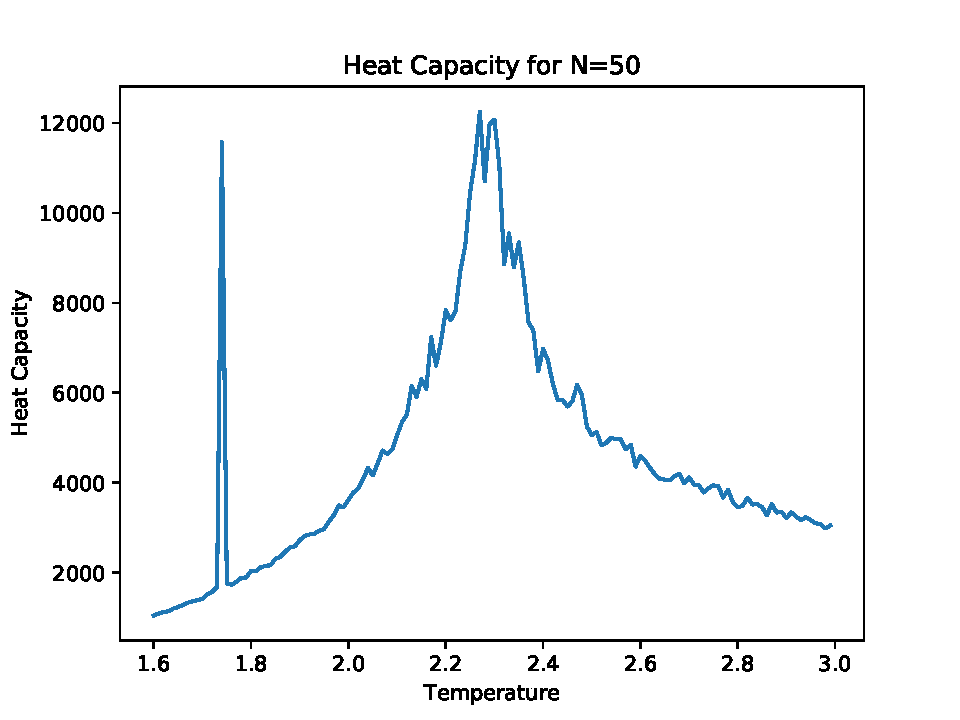
\includegraphics[width=.3\textwidth]{../figs/q4_N50_C.pdf}
\end{center}

We can see then that the Curie Temperature, at least as we can see from a $50x50$ lattice, is around $(2.28 - 2.31)$ $\frac{J}{k_b}$. We can also see that the clearest signature of the transistion is at the magnetic susceptibility with the Heat capacity being a close second.
\end{document}
